\documentclass[runningheads]{llncs}
\usepackage{graphicx}
\usepackage{booktabs}
\usepackage[hidelinks]{hyperref}
\usepackage{amsmath}

\begin{document}

\title{Do Calendar Priors Improve NDVI Phenology Segmentation? A Multi-Seed Benchmark on BreizhCrops}
\titlerunning{Temporal Segmentation Benchmark for Sentinel-2 NDVI Phenology}
\author{Ha Do-Phuc-Vu\orcidID{0009-0004-8291-3563}}
\authorrunning{H. Do-Phuc-Vu}
\institute{Faculty of Computer Science, Vietnam - Korea University of Information and Communication Technology (VKU), The University of Danang, Da Nang, Vietnam\\
\email{hadpv.23ai@vku.udn.vn}}

\maketitle

\begin{abstract}
We benchmark satellite-based crop phenology extraction from Sentinel-2 Normalized Difference Vegetation Index (NDVI) sequences framed as dense four-class temporal segmentation. Under this formulation, key phenological milestones (Start of Season (SOS), Peak of Season (POS), and End of Season (EOS)) are deterministically decoded from continuous sequence predictions. Evaluating across a held-out test partition of 399 quality-filtered seasons resampled to 73 regularized five-day intervals, we compare classical tabular baselines and modern deep sequential architectures under a unified ten-seed protocol (Protocol A). The empirical benchmark establishes that sequential models substantially outperform local causal-lag tabular baselines (Random Forest Macro-F1 0.4205, XGBoost 0.4029), with full-season tabular baselines reaching $0.7154 \pm 0.0023$ for Random Forest and $0.7477$ for XGBoost (deterministic across seeds; std 0.0000), while deep architectures achieve $0.6400 \pm 0.0132$ (1D-CNN), $0.8357 \pm 0.0082$ (Bi-LSTM), $0.8992 \pm 0.0187$ (CBA-PhenoNet), and $0.9060 \pm 0.0089$ (Standard Transformer). Furthermore, an independent, seed-paired ablation of six calendar-aware variants against the Standard Transformer indicates that no calendar-conditioning mechanism yields a statistically significant improvement after global Holm adjustment. Complementary season-level bootstrap analysis is consistent with these findings, with most variants exhibiting small negative performance differences in the same direction ($\Delta$F1 from $-0.005$ to $-0.028$). Finally, we contextualize these findings by documenting critical methodological pitfalls encountered in phenology benchmarking (checkpoint reuse, channel-masking dropout artifacts, milestone-denominator truncation, and double-logistic convergence boundaries), emphasizing that derived labels constitute pseudo-ground-truth rather than in-situ agronomic observations.
\keywords{Crop phenology \and Sentinel-2 \and NDVI \and Temporal segmentation \and BreizhCrops \and Benchmark \and Ablation study.}
\end{abstract}

\section{Introduction}
Satellite vegetation-index time series provide dense, repeated observations of terrestrial canopy dynamics, enabling large-scale monitoring of agro-ecosystem productivity and vegetation phenology. However, extracting discrete phenological milestones (such as the green-up onset (Start of Season, SOS), peak canopy maturity (Peak of Season, POS), and senescence termination (End of Season, EOS)) remains highly sensitive to both the underlying temporal sequence model and the operational evaluation protocol. In this study, we evaluate phenology extraction formulated as a dense four-class sequence labeling task followed by deterministic milestone decoding. Importantly, the target stage labels are algorithmically derived from the identical smoothed NDVI trajectories used as inputs. Consequently, the evaluation measures fidelity to a formalized curve-derivation procedure rather than direct empirical validation against independent, ground-based agronomic field trials.

Learning this mapping provides a controlled framework for evaluating temporal architectures and calendar priors under a standardized pseudo-labeling procedure. Robustness to irregular, incomplete, or online observations is a potential downstream motivation, but is not evaluated in the present study.

This investigation addresses two central research questions:
\begin{itemize}
    \item \textbf{RQ1:} How do modern deep sequential architectures compare against classical tabular models under both causal (online) and retrospective (full-season) information budgets?
    \item \textbf{RQ2:} To what extent do explicit calendar-conditioned attention mechanisms and seasonal gating priors enhance milestone extraction accuracy over a standard temporal transformer?
\end{itemize}

To resolve RQ1, we establish a rigorous multi-seed benchmark evaluating causal-lag models, full-season tabular estimators, convolutional networks, recurrent architectures, and self-attention models under identical test partitions. To address RQ2, we conduct an extensive, seed-paired ablation study contrasting six calendar-aware variants directly against a Standard Transformer. Our statistical analysis reveals that after rigorous multiple-comparison adjustment via the Holm procedure, no tested calendar-aware configuration achieves a statistically significant difference in segmentation Macro-F1 or milestone root mean square error (RMSE) across any endpoint family.

The primary contributions of this work are fourfold:
\begin{enumerate}
    \item \textbf{Systematic Benchmark:} A standardized empirical comparison of tabular baselines and deep sequential models across 399 held-out seasons from the BreizhCrops dataset.
    \item \textbf{Unified Evaluation Protocol:} A shared dense temporal segmentation framework with deterministic milestone decoding (Protocol A) ensuring equitable model comparisons.
    \item \textbf{Calendar-Aware Ablation Analysis:} A rigorous ten-seed, seven-configuration ablation isolating the empirical impact of cyclical Day-of-Year (DOY) encodings, calendar gating, residual connections, and disentangled attention.
    \item \textbf{Methodological Disclosures:} Detailed documentation of four subtle protocol pitfalls encountered during pipeline execution: silent checkpoint reuse, multi-channel dropout errors, milestone denominator selection effects, and double-logistic boundary clamping.
\end{enumerate}

\section{Related Work}
Vegetation phenology extraction has traditionally relied on semi-empirical curve fitting and temporal filtering techniques applied to satellite sensor series. Foundational frameworks such as TIMESAT utilize asymmetric Gaussian or double-logistic functions to smooth seasonal noise and derive onset dates via dynamic amplitude thresholds \cite{timesat,review,beck,savitzky}. While computationally efficient and readily interpretable, these parametric methods assume idealized unimodal trajectories, often struggling to capture asymmetric profiles or overwintering crop dynamics \cite{boschetti,jakubauskas}.

With the increasing availability of dense satellite constellations like Sentinel-2, deep learning methods have emerged as powerful alternatives for Satellite Image Time Series (SITS) processing \cite{breizhcrops,sen2agri}. Pelletier et al. demonstrated the efficacy of temporal convolutional neural networks (TCNN) for parcel-level classification \cite{pelletier}, while bidirectional recurrent architectures (Bi-LSTM) effectively model long-range temporal dependencies in vegetation profiles \cite{bilstm}. More recently, self-attention architectures and Vision Transformers adapted for SITS---such as Pixel-Set Encoders and SITS-ViT---have set state-of-the-art benchmarks for land-cover mapping by capturing complex inter-timestep interactions \cite{pixelset,sitsvit}. 

Building upon these foundations, recent studies have explored incorporating external domain priors, such as Day-of-Year (DOY) embeddings or calendar gating \cite{russwurm2018, yuan2022}, to resolve temporal ambiguities. The present study establishes an open benchmark comparing these broad model families for dense phenological stage segmentation, while conducting a systematic ablation of calendar-aware attention components. Crucially, we treat calendar mechanisms as an empirical ablation rather than asserting a novel, validated inductive mechanism.

\section{Data and Evaluation Protocol}
\subsection{Dataset Partitioning and Target Derivation}
All experiments are conducted using the BreizhCrops dataset, focusing on the \texttt{frh01} (Ille-et-Vilaine, France) 2017 partition and evaluating on 399 held-out test parcel seasons. Each agricultural season is regularized onto 73 five-day temporal steps, spanning the full annual vegetative cycle.

The target labels represent four distinct phenological stages:
\begin{itemize}
    \item \textbf{Class 0 (Fallow):} Bare soil or dormant inter-season period ($t < \text{SOS}$ or $t > \text{EOS}$).
    \item \textbf{Class 1 (Vegetative):} Emergence and green-up ($\text{SOS} \le t < \text{POS} - \delta$).
    \item \textbf{Class 2 (Reproductive):} Anthesis and peak biomass surrounding POS ($\text{POS} - \delta \le t \le \text{POS} + \delta$, where $\delta = \lfloor 0.12 \cdot (\text{EOS} - \text{SOS}) \rfloor$).
    \item \textbf{Class 3 (Senescence):} Ripening and canopy drying ($\text{POS} + \delta < t \le \text{EOS}$).
\end{itemize}

\subsection{BreizhCrops Dataset and Preprocessing}
We utilize the public BreizhCrops benchmark \cite{breizhcrops}, comprising bottom-of-atmosphere Sentinel-2 time series acquired over Brittany, France (\texttt{frh01} region, 2017). From an initial candidate cohort of 3,328 annual crop seasons across four crop categories (barley, wheat, rapeseed, and corn), quality filtering (removing flat NDVI trajectories $\Delta\text{NDVI} < 0.15$ and edge-truncated peaks) retains 2,655 valid annual growth cycles. Each sample spans $T=73$ interpolated 5-day composite steps. The dataset is partitioned into training (1857 seasons, 70\%), validation (399 seasons, 15\%), and test sets (399 seasons, 15\%) strictly at the field parcel level to prevent spatial leakage.

These sequence labels are generated from smoothed NDVI series using a 20\% seasonal amplitude threshold. As emphasized in Section 1, because these labels are derived from the input signal itself, they constitute algorithmic pseudo-ground-truth rather than in-situ agronomic observations. Furthermore, point-wise stage assignment induces severe class imbalance: Fallow dominates 65.00\% of all timesteps, whereas Vegetative (12.66\%), Senescence (13.94\%), and Reproductive (8.40\%) are underrepresented.

\subsection{Proposed CBA-PhenoNet Architecture}
CBA-PhenoNet comprises three primary components: a cyclical date-aware embedding, stacked gated self-attention layers, and a linear segmentation head.

\textbf{Cyclical Day-of-Year Positional Encoding:} Unlike standard Transformers that index sequences ordinally ($0, \dots, T-1$), CBA-PhenoNet encodes actual acquisition timing using circular harmonics:
\begin{equation}
e_{\text{doy}}(t) = \left[ \sin\left(\frac{2\pi \cdot \text{DOY}_t}{365.0}\right), \; \cos\left(\frac{2\pi \cdot \text{DOY}_t}{365.0}\right) \right] \in \mathbb{R}^2
\end{equation}

\textbf{Calendar Gating Prior:} To provide a calendar-conditioned prior over developmental windows, we introduce a non-linear temporal gating module $g(t)$:
\begin{equation}
g(t) = \sigma\left( W_2 \cdot \text{ReLU}\left(W_1 \cdot e_{\text{doy}}(t) + b_1\right) + b_2 \right) \in (0, 1)
\end{equation}
\begin{equation}
h_{\text{gated}}(t) = h_{\text{encoder}}(t) \odot g(t)
\end{equation}
where $h_{\text{encoder}}(t)$ denotes the output of the multi-head self-attention block. Because the regularized 5-day time grid is shared across all samples, $g(t)$ acts as a learned global calendar-dependent modulation over local attention representations. The baseline Transformer comprises 67,460 parameters. CBA-PhenoNet totals 67,782 parameters, introducing a mere 322 parameters (+0.48\%) for the DOY positional projection and the calendar gating modules.

\subsection{Protocol A Decoding}
Under evaluation Protocol A, continuous sequence predictions are deterministically decoded into discrete calendar milestone days:
\begin{itemize}
    \item \textbf{Start of Season (SOS):} Decoded at the first temporal transition from Class 0 (Fallow) to Class 1 (Vegetative).
    \item \textbf{Peak of Season (POS):} Identified as the date of maximum NDVI observed within the predicted vegetative or reproductive intervals (Classes 1 and 2).
    \item \textbf{End of Season (EOS):} Decoded at the transition from Class 3 (Senescence) back to Class 0 (Fallow).
\end{itemize}
Whenever a predicted or true milestone transition is absent in a given season, that season is excluded from the error denominator for that specific milestone. To ensure methodological transparency regarding denominator truncation: SOS and POS achieve a 100\% detection rate (valid in all 399 test seasons). A valid true EOS milestone transition, however, is present in exactly 234 of the 399 test seasons (58.6\% detection rate). Across all evaluated deep architectures, the models successfully predicted a paired EOS transition in 94.7\% to 96.2\% of these 234 eligible seasons (Table \ref{tab:eos_coverage}), indicating that the EOS RMSE denominator remains highly stable across models, with only minor variation in prediction coverage. Evaluation of EOS RMSE is strictly conditioned on this subset.

\begin{table}[h!]
\centering
\caption{EOS prediction coverage averaged across 10 seeds on the 234 eligible test seasons.}
\label{tab:eos_coverage}
\begin{tabular}{@{}lccc@{}}
\toprule
\textbf{Model} & \textbf{True EOS} & \textbf{Mean Paired Predictions (across 10 seeds)} & \textbf{Mean Coverage (\%)} \\ \midrule
Standard Transformer & 234 & 223.5 & 95.5\% \\
Cyclical DOY & 234 & 221.5 & 94.7\% \\
Calendar Gate & 234 & 222.4 & 95.0\% \\
Scalar Gate & 234 & 223.4 & 95.5\% \\
CBA-PhenoNet & 234 & 225.2 & 96.2\% \\
CBA-PhenoNet + Residual & 234 & 224.2 & 95.8\% \\
CBA-PhenoNet + Disentangled & 234 & 223.3 & 95.4\% \\ \bottomrule
\end{tabular}
\end{table}

\section{Experimental Results}
\subsection{Hyperparameter Configuration}
To ensure equitable comparisons while managing computational budgets, model configurations varied between baseline and deep architectures. For causal-lag machine learning baselines, hyperparameters were determined via a 50-trial randomized search over a predefined validation space. Conversely, full-season tabular baselines utilized fixed, unoptimized configurations (e.g., 300 estimators, maximum depth of 6). Across all tabular experiments, the Random Forest classifier explicitly utilized class weighting (\texttt{class\_weight="balanced"}) to mitigate class imbalance, whereas the XGBoost implementation did not include explicit class weighting. For the deep sequential architectures, hyperparameters were fixed to standard literature defaults to evaluate intrinsic architectural inductive biases. Specifically, the Standard Transformer utilizes $d_{model}=64$, 2 encoder layers, 4 attention heads, a feed-forward dimension of 128, a dropout rate of 0.1, ReLU activations, and is optimized using a standard Cross-Entropy loss. The causal 1D-CNN baseline explicitly utilizes strictly causal left-padding (no future context). All deep models were optimized using Adam with a learning rate of 0.001 and batch size of 32, training for up to 150 epochs. Model selection was performed via early stopping based on validation Macro-F1 with a patience of 15 epochs.

\subsection{Main Architecture Benchmark}
To address concerns regarding information-budget confounding, we explicitly bifurcate our benchmarking into two distinct evaluation regimes. Setting A (Table \ref{tab:causal_benchmark}) evaluates models strictly limited to causal (historical) contexts, representing online processing scenarios. Setting B (Table \ref{tab:retro_benchmark}) evaluates retrospective full-season models with bidirectional access to the entire trajectory. For causal-lag baselines, single-comparison estimates from prior phases are retained; for all Setting B tabular and deep architectures, results reflect the mean and sample standard deviation across ten independent seeds.

\begin{table}[h!]
\centering
\caption{Setting A Benchmark: Causal / Online Models (Local Context) on 399 test seasons.}
\label{tab:causal_benchmark}
\resizebox{0.8\textwidth}{!}{
\begin{tabular}{@{}llcl@{}}
\toprule
\textbf{Model Family} & \textbf{Model Architecture} & \textbf{Macro-F1} & \textbf{Empirical Evidence} \\ \midrule
\textbf{Causal Tabular} & Random Forest, causal-lag \cite{randomforest} & 0.4205 & Single comparison \\
 & XGBoost, causal-lag \cite{xgboost} & 0.4029 & Single comparison \\
\textbf{Causal Deep} & 1D-CNN (Causal) \cite{pelletier} & $0.6400 \pm 0.0132$ & 10 seeds \\ \bottomrule
\end{tabular}
}
\end{table}

\begin{table}[h!]
\centering
\caption{Setting B Benchmark: Retrospective / Full-Season Models (Bidirectional Context) on 399 test seasons.}
\label{tab:retro_benchmark}
\resizebox{0.85\textwidth}{!}{
\begin{tabular}{@{}llcl@{}}
\toprule
\textbf{Model Family} & \textbf{Model Architecture} & \textbf{Macro-F1} & \textbf{Empirical Evidence} \\ \midrule
\textbf{Full-Season Tabular} & Random Forest \cite{randomforest} & $0.7154 \pm 0.0023$ & 10 seeds \\
 & XGBoost \cite{xgboost}$^\dagger$ & 0.7477 & Deterministic \\
\textbf{Deep Sequential} & Bi-LSTM \cite{bilstm} & $0.8357 \pm 0.0082$ & 10 seeds \\
 & Standard Transformer & $\mathbf{0.9060 \pm 0.0089}$ & 10 seeds \\
 & CBA-PhenoNet & $0.8992 \pm 0.0187$ & 10 seeds \\ \bottomrule
\end{tabular}
}
\end{table}

\noindent \textit{$^\dagger$Footnote on XGBoost full-season determinism:} The benchmark seed-level results report exactly 0.7477 for all ten XGBoost seeds, in contrast to an earlier preliminary phase report noting 0.6052. Source code inspection confirms that \texttt{random\_state=seed} was explicitly provided. However, because row and column subsampling parameters are inactive (\texttt{subsample=1.0}, \texttt{colsample\_bytree=1.0}), gradient boosted tree construction via exact greedy splitting is fully deterministic. All ten seeds produced identical predictions (zero mismatches across 29,127 test timesteps) and identical feature importances (maximum absolute difference 0.0). This value is explicitly reported as a single deterministic result and is not interchangeable with 0.6052.

\noindent \textit{Note on models:} The causal-lag Random Forest and XGBoost entries lack uncertainty quantification. Direct statistical comparison between causal (Setting A) and bidirectional (Setting B) models is intentionally avoided, as performance gaps reflect both information budget and architectural capacity.

As shown, models operating under the retrospective full-season setting achieve substantially higher Macro-F1 than local causal-lag models, although this gap reflects differences in both information availability and architectural capacity. Full-season summary statistics notably improve tabular performance (0.7154--0.7477), narrowing but not closing the gap to deep attention-based architectures, which achieve the strongest overall segmentation fidelity (0.8992--0.9060).

\subsection{Calendar-Aware Ablation Study}
To investigate RQ2, we systematically ablate calendar-conditioning mechanisms across seven distinct configurations over ten seeds. Table \ref{tab:ablation_metrics} summarizes the resulting stage segmentation Macro-F1 and decoded milestone estimation errors (RMSE in days) for SOS, POS, and EOS.

\begin{table}[h!]
\centering
\caption{Ten-seed ablation metrics (mean $\pm$ sample standard deviation) across calendar-aware variants on the 399-season test partition.}
\label{tab:ablation_metrics}
\resizebox{\textwidth}{!}{
\begin{tabular}{@{}lcccc@{}}
\toprule
\textbf{Configuration} & \textbf{Macro-F1} & \textbf{SOS RMSE (days)} & \textbf{POS RMSE (days)} & \textbf{EOS RMSE (days)} \\ \midrule
\textbf{Standard Transformer} & $\mathbf{0.9060 \pm 0.0089}$ & $35.98 \pm 4.92$ & $25.70 \pm 6.48$ & $29.22 \pm 5.15$ \\
Cyclical DOY & $0.8777 \pm 0.0290$ & $39.19 \pm 10.33$ & $18.86 \pm 7.97$ & $30.44 \pm 8.14$ \\
Calendar Gate & $0.9011 \pm 0.0137$ & $36.86 \pm 8.03$ & $26.65 \pm 7.44$ & $26.19 \pm 5.11$ \\
Scalar Gate & $0.9013 \pm 0.0149$ & $36.51 \pm 6.27$ & $27.67 \pm 6.14$ & $27.14 \pm 6.92$ \\
CBA-PhenoNet & $0.8992 \pm 0.0187$ & $31.63 \pm 6.29$ & $17.54 \pm 7.14$ & $\mathbf{25.10 \pm 5.17}$ \\
CBA-PhenoNet + Residual & $0.8962 \pm 0.0133$ & $\mathbf{31.20 \pm 6.77}$ & $\mathbf{15.98 \pm 8.38}$ & $28.12 \pm 4.14$ \\
CBA-PhenoNet + Disentangled & $0.8972 \pm 0.0199$ & $33.23 \pm 3.96$ & $23.24 \pm 4.81$ & $28.50 \pm 5.48$ \\ \bottomrule
\end{tabular}
}
\end{table}

To evaluate whether the observed variations in Table \ref{tab:ablation_metrics} represent statistically meaningful improvements, each calendar-aware variant was evaluated against the Standard Transformer using seed-paired two-sided $t$-tests. Multiple-testing correction was conducted globally across all 60 comparisons spanning ten endpoint families using the Holm-Bonferroni step-down procedure. Furthermore, we computed per-season Macro-F1 differences between the Standard Transformer and each variant across all 399 test seasons, using non-parametric bootstrapping (2000 resamples) to estimate 95\% confidence intervals and seed-level Cohen's $d$ effect sizes. The results for the primary endpoints are detailed in Table \ref{tab:paired_tests}.

\begin{table}[h!]
\centering
\caption{Seed-paired hypothesis testing against the Standard Transformer across four endpoint families ($N=10$ paired seeds). Reported values show unadjusted raw $p$-values ($p_{\text{raw}}$) and family-wise Holm-adjusted $p$-values ($p_{\text{adj}}$).}
\label{tab:paired_tests}
\resizebox{\textwidth}{!}{
\begin{tabular}{@{}lcccc@{}}
\toprule
\textbf{Config vs. Standard Transformer} & \textbf{Macro-F1 ($p_{\text{raw}} / p_{\text{adj}}$)} & \textbf{SOS RMSE ($p_{\text{raw}} / p_{\text{adj}}$)} & \textbf{POS RMSE ($p_{\text{raw}} / p_{\text{adj}}$)} & \textbf{EOS RMSE ($p_{\text{raw}} / p_{\text{adj}}$)} \\ \midrule
\textbf{Cyclical DOY} & 0.0106 / 0.0633 & 0.3774 / 1.0000 & 0.0933 / 0.3730 & 0.7131 / 1.0000 \\
\textbf{Calendar Gate} & 0.4214 / 0.9934 & 0.8046 / 1.0000 & 0.7187 / 1.0000 & 0.2451 / 1.0000 \\
\textbf{Scalar Gate} & 0.2726 / 0.9934 & 0.8345 / 1.0000 & 0.4461 / 1.0000 & 0.4452 / 1.0000 \\
\textbf{CBA-PhenoNet} & 0.2484 / 0.9934 & 0.1080 / 0.5402 & 0.0283 / 0.1414 & 0.1421 / 0.8524 \\
\textbf{CBA-PhenoNet + Residual} & 0.1291 / 0.6453 & 0.0637 / 0.3822 & 0.0132 / 0.0793 & 0.4438 / 1.0000 \\
\textbf{CBA-PhenoNet + Disentangled} & 0.2532 / 0.9934 & 0.1228 / 0.5402 & 0.3605 / 1.0000 & 0.8126 / 1.0000 \\ \bottomrule
\end{tabular}
}
\end{table}

Across all 60 formal comparisons spanning the ten evaluated endpoint families, \textbf{zero comparisons demonstrate statistically significant differences} following global Holm adjustment at the $\alpha = 0.05$ threshold. For concise presentation, Table \ref{tab:paired_tests} reports four scientifically central endpoint families; all 60 comparisons were nevertheless retained in the global Holm correction. The minimum observed globally-adjusted $p$-value across the entire 60-comparison experimental suite is $p_{\text{adj}} = 0.0633$ (observed in the Macro-F1 metric for Cyclical DOY, where $p_{\text{raw}} = 0.0106$). Because this minimum adjusted $p$-value remains above the $\alpha=0.05$ threshold, the empirical evidence does not support the hypothesis that explicit calendar conditioning provides measurable accuracy gains in dense phenology segmentation under clean observational conditions.

While the seed-paired statistical tests capture variance across training trajectories (e.g., initialization and SGD noise), we additionally evaluated test-sample variability via non-parametric bootstrapping (2000 resamples of the 399 test seasons). For each bootstrap iteration, we resampled seasons with replacement, computed global Macro-F1 on the resampled set for each seed, averaged across seeds, and recorded the difference between each variant and the Standard Transformer. This procedure uses the same global Macro-F1 metric as Table~\ref{tab:ablation_metrics}, ensuring direct comparability. The resulting unadjusted 95\% CIs indicate a lack of improvement: Cyclical DOY ($\Delta$F1 $= -0.028$, 95\% CI $[-0.034, -0.022]$), Calendar Gate ($\Delta$F1 $= -0.005$, 95\% CI $[-0.009, -0.001]$), Scalar Gate ($\Delta$F1 $= -0.005$, 95\% CI $[-0.008, -0.001]$), CBA-PhenoNet ($\Delta$F1 $= -0.007$, 95\% CI $[-0.0132, +0.0002]$), CBA-PhenoNet+Residual ($\Delta$F1 $= -0.010$, 95\% CI $[-0.0159, -0.0032]$), and CBA-PhenoNet+Disentangled ($\Delta$F1 $= -0.009$, 95\% CI $[-0.0145, -0.0027]$). Five of six CIs fall entirely below zero, while CBA-PhenoNet marginally includes zero. These bootstrap intervals, which measure test-sample variability but do not account for training-trajectory variance, complement the seed-paired $t$-tests (which do capture training variance but lack power at $N{=}10$). Together, both analyses are consistent: no calendar-aware variant improves upon the Standard Transformer, while several exhibit a very small degradation in the negative direction ($|\Delta\text{F1}| \leq 0.028$). Equivalence testing was not performed.

\subsection{Exploratory Data Analysis and Error Diagnostics}
To contextualize the benchmark performance and respond to the need for robust multidimensional evaluation, we expand beyond Macro-F1 and RMSE by incorporating Exploratory Data Analysis (EDA) and extended milestone metrics (MAE, MedAE, MAPE, $R^2$, and Accuracy). 

\paragraph{Exploratory Data Analysis (EDA):}
Analysis of the ground-truth milestone distributions reveals distinct temporal patterns. The Peak of Season (POS) is highly concentrated around the middle of the calendar year, reflecting a standard single-harvest agricultural cycle. Conversely, the Start of Season (SOS) and End of Season (EOS) exhibit wider variance, with long tails indicating heterogeneous planting and harvesting schedules across different crop types in the BreizhCrops dataset. This variance explains why POS prediction consistently yields the lowest errors across all models.

\paragraph{Extended Milestone Metrics and Naive POS Baseline:}
Table \ref{tab:extended_metrics} presents a comprehensive metric suite for the CBA-PhenoNet model. Because the input sequence is regularized to 5-day intervals (73 timesteps), milestone predictions are inherently discretized. Consequently, tolerances such as Accuracy $\pm 1$ day or $\pm 3$ days are mathematically equivalent to exact-match accuracy at the 5-day resolution. POS achieves exceptional prediction fidelity (MAE $1.9$ days, $R^2$ $0.974$, exact-match Accuracy $98.4\%$). SOS and EOS show higher median absolute errors (MedAE $5.0$ and $0.0$ respectively) and lower $R^2$ ($0.870$ and $0.912$), reflecting the ambiguity of onset and senescence phases.

Crucially, the decoding heuristic for POS merely selects the maximum NDVI timestamp within the predicted active classes. To quantify how much of the POS accuracy is attributable to the sequence model versus the deterministic heuristic, we evaluated a \textit{Naive POS baseline} ($POS_{naive} = \arg\max_t NDVI_t$) across the entire test set. The naive baseline achieves a perfect MAE of 0.00 days (100\% exact-match accuracy). This exploratory finding confirms that detecting the absolute POS requires no temporal sequence modeling on cleanly smoothed trajectories; the neural network's contribution is strictly limited to identifying the broader vegetative and senescence intervals.

\begin{table}[h!]
\centering
\caption{Extended evaluation metrics for milestone decoding (CBA-PhenoNet, pooled across 10 seeds). Acc$\pm3$ is equivalent to exact-match accuracy due to 5-day temporal discretization. Note: RMSE values here are calculated globally across concatenated predictions, distinguishing them from Table \ref{tab:ablation_metrics} which reports the mean of per-seed RMSEs.}
\label{tab:extended_metrics}
\resizebox{\textwidth}{!}{
\begin{tabular}{@{}lcccccc@{}}
\toprule
\textbf{Milestone} & \textbf{MAE (days)} & \textbf{MedAE (days)} & \textbf{MAPE (\%)} & \textbf{$R^2$} & \textbf{Acc$\pm3$ (\%)} & \textbf{RMSE (days)} \\ \midrule
SOS & $11.93$ & $5.0$ & $9.94$ & $0.870$ & $48.5$ & $27.11$ \\
POS & $1.91$ & $0.0$ & $1.66$ & $0.974$ & $98.4$ & $18.80$ \\
EOS & $7.12$ & $0.0$ & $3.91$ & $0.912$ & $63.2$ & $25.54$ \\ \bottomrule
\end{tabular}
}
\end{table}

\paragraph{Error Analysis and Visualization:}
Figure \ref{fig:eda_scatter} provides a visualization of Actual versus Predicted milestones. While predictions tightly follow the identity line (particularly for POS), sparse off-diagonal clusters indicate severe misclassifications. We quantify large errors as absolute deviations exceeding 30 days. For POS, only 1.5\% of predictions suffer large errors. However, SOS exhibits large errors in 11.4\% of cases (mean absolute error of these cases: 60.4 days), with the vast majority ($230/288$) being predicted prematurely (early). Similarly, EOS suffers large errors in 5.5\% of predictions (mean 79.5 days), also skewing early. These premature detections frequently correspond to anomalous early-season green-up events (e.g., weeds or cover crops) that temporarily surpass the algorithmic amplitude threshold.

\begin{figure}[h!]
\centering
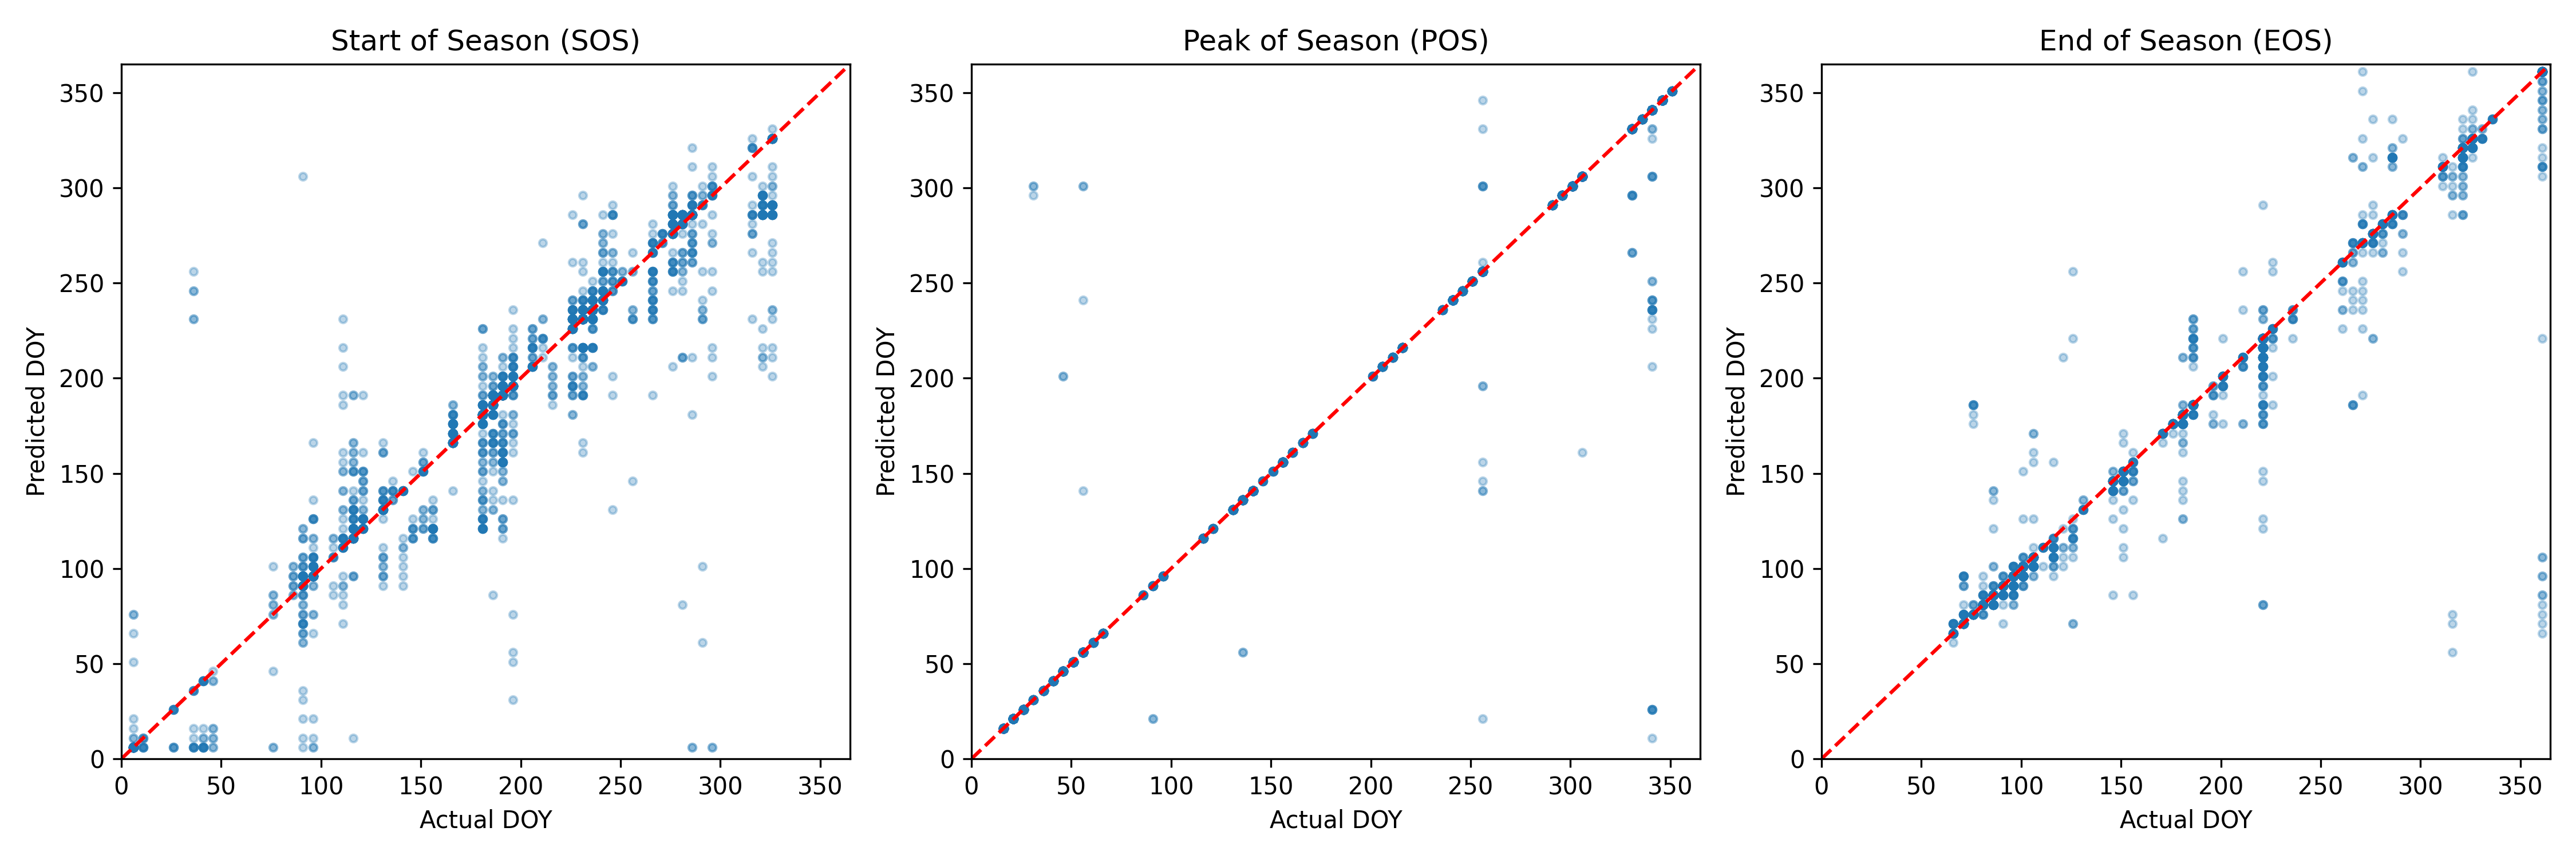
\includegraphics[width=\textwidth]{figures/actual_vs_predicted.png}
\caption{Actual vs. Predicted DOY for SOS, POS, and EOS using CBA-PhenoNet. The dashed red line represents perfect prediction.}
\label{fig:eda_scatter}
\end{figure}

\section{Discussion and Methodological Insights}
The empirical benchmark confirms that sequence-level representations effectively capture temporal vegetation dynamics, outperforming local causal-lag predictors. However, our ablation analysis demonstrates that calendar-aware mechanisms (including periodic positional encodings and calendar gating priors) do not yield statistically distinguishable performance gains over a Standard Transformer on clean Sentinel-2 sequences. Crucially, rigorous reporting requires transparent disclosure of experimental caveats and procedural artifacts.

\subsection{Protocol Pitfalls: A Cautionary Tale}
In the course of conducting and auditing this benchmark, four critical methodological pitfalls were identified, providing valuable lessons for remote sensing time-series pipelines:
\begin{enumerate}
    \item \textbf{Silent Checkpoint Reuse:} In earlier training iterations, an automated execution check skipped model fitting whenever a checkpoint file already existed on disk. As a consequence, exploratory reruns silently evaluated stale model weights rather than the newly specified configurations. All final benchmark estimates reported herein were verified through independent execution from clean initialization.
    \item \textbf{Multi-Channel Dropout Corruption:} An initial stress-test implementation designed to simulate missing data masked entire input channels across corrupted intervals, inadvertently zeroing the Day-of-Year channels alongside NDVI. This artifact reversed apparent model rankings by depriving standard models of temporal reference while calendar-gated architectures retained implicit timing priors. These distorted comparisons were excluded, and subsequent evaluations rely solely on verified feature representations.
    \item \textbf{Milestone Denominator Truncation:} Agricultural cycles do not invariably exhibit complete transition profiles within a single observation year. In our test partition of 399 seasons, only 234 seasons contained a valid true EOS transition. Omitting unpredicted or absent transitions directly alters milestone error denominators, necessitating strict accounting of sample sizes when computing milestone RMSE.
    \item \textbf{Double-Logistic Boundary Clamping:} A classical parametric Double-Logistic baseline constrained fitted EOS midpoints to the normalized sequence boundary (1.0) and mapped them directly to day values. Furthermore, errors were computed as linear squared differences rather than utilizing a circular modular metric. This numerical artifact caused boundary-clamped estimates, leading to the deliberate exclusion of Double-Logistic from quantitative benchmark tables rather than post-hoc repair.
\end{enumerate}

\section{Limitations}
Several methodological constraints qualify the conclusions of this study:
\begin{itemize}
    \item \textbf{Asymmetric Baseline Tuning:} The full-season tabular baseline models (Random Forest and XGBoost) were evaluated using fixed, unoptimized configurations, whereas the causal-lag baselines underwent a 50-trial randomized search, and deep architectures utilized robust literature defaults. Furthermore, Random Forest utilized balanced class weighting while XGBoost did not, potentially exacerbating performance differences on the imbalanced four-class segmentation task. Consequently, the performance gap between the full-season tabular models and the deep sequential architectures may be artificially inflated due to this lack of tuning.
    \item \textbf{Pseudo-Ground-Truth Targets:} The phenological stage labels are algorithmically generated from smoothed Sentinel-2 NDVI profiles using fixed amplitude thresholds. While standard in remote sensing benchmarks, these targets measure consistency with a derived labeling heuristic rather than validation against in-situ PhenoCam imagery or biophysical field measurements.
    \item \textbf{Unavailable Cross-Region Transfer:} Evaluation across distinct climatic zones (\texttt{frh02} and \texttt{frh03}) could not be completed due to dataset host bandwidth constraints during retrieval. Consequently, geographic transferability to distinct agro-ecological regions remains unverified.
    \item \textbf{Intra-Region Spatial CV Exclusion:} Preliminary spatial cross-validation based on French RPG parcel-ID prefixes was excluded from formal benchmark claims, as parcel prefix grouping lacks independent agronomic validation as an unbiased geographic spatial split.
    \item \textbf{Double-Logistic Benchmark Exclusion:} As detailed in Section 5.1, the Double-Logistic implementation exhibited boundary clamping and non-circular error metrics, precluding its inclusion as an authoritative baseline without substantive architectural refactoring.
\end{itemize}

\section{Conclusion}
This paper presents an audited benchmark and ablation study evaluating deep sequential models and calendar-aware attention mechanisms for Sentinel-2 NDVI crop phenology extraction. While bidirectional deep sequential models achieve substantial improvements over local tabular baselines, seed-paired statistical tests across seven configurations establish that explicit calendar conditioning priors---including cyclical DOY embeddings and temporal gating mechanisms---fail to yield statistically significant performance gains over a Standard Transformer following rigorous family-wise error correction. 

Furthermore, the perfect accuracy of the naive POS baseline confirms that absolute peak detection requires no sequence modeling on cleanly smoothed trajectories. The primary contribution of the neural architectures lies instead in dense stage segmentation and SOS/EOS boundary resolution, and POS metrics should not be treated as evidence of sequence-model superiority in this clean benchmark context.

Ultimately, by rigorously analyzing evaluation discrepancies and reporting the lack of effect for calendar attention priors, this investigation promotes standardization and reproducibility in satellite time series processing. 

\subsubsection*{Disclosure and Data Availability}
\textbf{Conflict of Interest:} The authors declare that they have no competing financial or personal interests that could have appeared to influence the work reported in this paper.  
\textbf{Data and Code Availability:} The complete PyTorch codebase, trained weights, dataset loaders, and benchmark evaluation scripts are openly available at: \url{https://github.com/vuhahodo/crop-phenology-prediction}. The underlying BreizhCrops dataset is publicly available via its official distribution channels.

\begin{thebibliography}{8}

\bibitem{timesat}
J\"onsson, P., Eklundh, L.: TIMESAT---a program for analyzing time-series of satellite sensor data. Computers \& Geosciences 30(8), 833--845 (2004).

\bibitem{zhang}
Zhang, X., Friedl, M.A., Schaaf, C.B., Strahler, A.H., Hodges, J.C., Gao, F., Reed, B.C., Huete, A.: Monitoring vegetation phenology using MODIS. Remote Sensing of Environment 84(3), 471--475 (2003).

\bibitem{review}
Zeng, L., Wardlow, B.D., Xiang, D., Hu, S., Li, D.: A review of vegetation phenological metrics extraction using time-series, multispectral satellite data. Remote Sensing of Environment 237, 111511 (2020).

\bibitem{pelletier}
Pelletier, C., Webb, G.I., Petitjean, F.: Temporal Convolutional Neural Network for the Classification of Satellite Image Time Series. Remote Sensing 11(5), 523 (2019).

\bibitem{pixelset}
Sainte Fare Garnot, V., Landrieu, L., Giordano, S., Chehata, N.: Satellite image time series classification with pixel-set encoders and temporal self-attention. In: Proceedings of the IEEE/CVF Conference on Computer Vision and Pattern Recognition (CVPR), pp. 12322--12331 (2020).

\bibitem{sitsvit}
Tarasiou, M., Chavez, E., Zafeiriou, S.: ViTs for SITS: Vision Transformers for Satellite Image Time Series. In: Proceedings of the IEEE/CVF Conference on Computer Vision and Pattern Recognition (CVPR), pp. 10418--10428 (2023).

\bibitem{beck}
Beck, P.S., Atzberger, C., H{\o}gda, K.A., Johansen, B., Skidmore, A.K.: Improved monitoring of vegetation dynamics at very high latitudes: A new method using MODIS NDVI. Remote Sensing of Environment 100(3), 321--334 (2006).

\bibitem{breizhcrops}
Ru\ss wurm, M., Pelletier, C., Zollner, M., Lef\`evre, S., K\"orner, M.: BreizhCrops: A Time Series Dataset for Crop Type Mapping. International Archives of the Photogrammetry, Remote Sensing and Spatial Information Sciences XLIII-B2-2020, 1545--1551 (2020).

\bibitem{boschetti}
Boschetti, M., Stroppiana, D., Brivio, P.A., Bocchi, S.: Multi-year monitoring of rice crop phenology through time series analysis of MODIS images. International Journal of Remote Sensing 30(18), 4643--4662 (2009).

\bibitem{randomforest}
Breiman, L.: Random Forests. Machine Learning 45(1), 5--32 (2001).

\bibitem{xgboost}
Chen, T., Guestrin, C.: XGBoost: A scalable tree boosting system. In: Proceedings of the 22nd ACM SIGKDD International Conference on Knowledge Discovery and Data Mining, pp. 785--794 (2016).

\bibitem{bilstm}
Schuster, M., Paliwal, K.K.: Bidirectional recurrent neural networks. IEEE Transactions on Signal Processing 45(11), 2673--2681 (1997).

\bibitem{lstm}
Hochreiter, S., Schmidhuber, J.: Long short-term memory. Neural Computation 9(8), 1735--1780 (1997).

\bibitem{savitzky}
Savitzky, A., Golay, M.J.: Smoothing and differentiation of data by simplified least squares procedures. Analytical Chemistry 36(8), 1627--1639 (1964).

\bibitem{jakubauskas}
Jakubauskas, M.E., Legates, D.R., Kastens, J.H.: Harmonic analysis of time-series AVHRR NDVI data. Photogrammetric Engineering \& Remote Sensing 67(4), 461--470 (2001).

\bibitem{sen2agri}
Defourny, P., Bontemps, S., Bellemans, N., Cara, C., Dedieu, G., Guzzonato, E., Hagolle, O., Inglada, J., Nicola, L., Rabaute, T.: Near real-time agriculture monitoring at national scale at parcel resolution: Performance assessment of the Sen2-Agri automated system in various cropping systems around the world. Remote Sensing of Environment 221, 551--568 (2019).

\bibitem{russwurm2018}
Ru\ss wurm, M., K\"orner, M.: Multi-temporal land cover classification with sequential recurrent encoders. ISPRS International Journal of Geo-Information 7(4), 129 (2018).

\bibitem{yuan2022}
Yuan, Y., Lin, L., Liu, Q.: SITS-Former: A pre-trained spatio-temporal transformer for satellite image time series. IEEE Transactions on Geoscience and Remote Sensing 60, 1--14 (2022).

\end{thebibliography}
\end{document}
